%
% body.tex
%
% Copyright © 2020 Libao Jin <jinlibao@outlook.com>
% Distributed under terms of the MIT license.
%
The deadline will be strictly enforced. If you do not submit in time there will be a $20\%$ penalty for each day you're late. Remember that you are allowed to work in teams of two on this assignment. You are encouraged to prepare your work in \LaTeX{}; a template will be provided to help you put it all together. If you choose  to submit a hard copy, you may submit only one copy for a team, indicating the names of both contributors. Online submission is encouraged, however, in that case both members of a team should submit the PDF file containing  their work and showing both their names.

\emph{All plots generated in this homework should have a title, legend, and labeled $x$ and $y$-axes.} \\[15pt]

\textbf{Instruction}

\begin{enumerate}[label={\arabic*.}]
  \item Go to \url{https://www.overleaf.com} and sign in (required).
  \item Open \href{https://www.overleaf.com/read/qdhgzdjpwbhj}{template}, click \emph{Menu} (up left corner), then \emph{Copy Project}.
  \item Go to \verb|LaTeX/meta.tex| (the file \verb|meta.tex| under the folder \verb|LaTeX|) to change the section and your name, e.g.,
    \begin{itemize}
      \item change title to \verb|\title{MATH 3340-01 Scientific Computing Homework 5}|
      \item change author to \verb|\author{Albert Einstein \& Carl F. Gauss}|
    \end{itemize}
  \item For Problem 2 and 3, you can encouraged to type the solution in \LaTeX{}. But if you want to write it on the printout, please make sure your scanned work is clear enough (failure to do so will lead to points deduction).
  \item For Problem 1, you need to write function/script files, store results to output files, and save graphs to figure files. Here are suggested names for function files, script files, output files, and figure files:
    \begin{table}[!hbtp]
      \centering
      % \caption{caption}
      % \label{tab:label}
      \begin{tabular}{cllll}
        \toprule
        Problem     & Function File     & Script File     & Output File       & Figure File         \\
        \midrule
        1(a)        & \verb|lagrange.m| & \verb|hw5_p1.m| &                   &                     \\
        1(b)        &                   &                 &                   & \verb|hw5_p1_b.pdf| \\
        1(c)        &                   &                 &                   & \verb|hw5_p1_c.pdf| \\
        \bottomrule
      \end{tabular}
    \end{table}

    Once finished, you need to upload these files to the folder \verb|src| on Overleaf. If you have different filenames, please update the filenames in \verb|\lstinputlisting{../src/your_script_name.m}| accordingly. You can code in the provided files in \href{https://libaoj.in/courses/2020f/MATH3340/Homework/5/hw5.zip}{hw5.zip}, and use the MATLAB script \verb|save_results.m| to generate the output files and store the graphs to \verb|.pdf| files automatically (the script filenames should be exactly same as listed above).
  \item Recompile, download and upload the generated PDF to WyoCourses.
  \item You may find \href{https://libaoj.in/files/LaTeX.Mathematical.Symbols.pdf}{\LaTeX{}.Mathematical.Symbols.pdf} and the second part of \href{https://libaoj.in/courses/2020f/MATH3341/slides/Math.3341.Lab.01.Slides.pdf}{Lab 01 Slides} and \href{https://libaoj.in/courses/2020f/MATH3341/slides/Math.3341.Lab.02.Slides.pdf}{Lab 02 Slides} helpful.
\end{enumerate}
\newpage

%%%%%%%%%%%%%%%%%%%%%%%%%%%%%%%%%%%%%%%%%%%%%%%%
% Problem 1
%%%%%%%%%%%%%%%%%%%%%%%%%%%%%%%%%%%%%%%%%%%%%%%%
\section{Problem 1}%
\label{sec:problem_1}
The purpose of this problem is two-fold. First we will construct an interpolating polynomial and compare this polynomial to the original function from which the data is extracted. Then we will investigate how the choice of nodes can affect the accuracy of a higher order interpolating polynomial.

You will notice that the interpolant will be  different depending on the number and type of nodes used. Contrary to our intuition, the use of higher order polynomials does not necessarily guarantee an increase in global accuracy unless careful judgement is exercised. This should become clear when examining the plots you will generate in this problem.

We will consider the function
\begin{equation*}
  f(x)
  = \frac{1}{1 + 16 x^{2}}
\end{equation*}
and construct the interpolating polynomial using the Lagrange interpolant formula given by
\begin{equation}
  \label{eq:lagrange}
  p(x)
  = \sum_{k = 0}^{n} y_{k} L_{k}(x),
  \quad \text{where $L_{k}(x) = \prod_{\substack{j = 0 \\ j \ne k}}^{n} \frac{x - x_{j}}{x_{k} - x_{j}}$}.
\end{equation}
Please note that you are not supposed to use the standard form of the polynomial. Use the Lagrange form instead, as indicated above.
\begin{enumerate}[label=(\alph*)]
  \item \label{enum:a} As usual, you will create a minimum of two code files for this problem: a function file, and a script file.
    \begin{enumerate}[label=(\roman*)]
      \item Write a function file, to be used in both part \ref{enum:b} and \ref{enum:c} below, that calculates the interpolating polynomial using the Lagrange interpolant in \eqref{eq:lagrange}. Your function file should have the inputs:
        \begin{lstlisting}[style=Plain,numbers=none]
xdata = the set of nodes x_k,
ydata = the values y_k = f(x_k),
x = the point, or set of points (fine grid), used to evaluate p(x)
        \end{lstlisting}
        and the output:
        \begin{lstlisting}[style=Plain,numbers=none]
p = the value(s) of p at the point (or set of points) x
        \end{lstlisting}
      \item Create a script file which will execute the steps outlined in parts \ref{enum:b} and \ref{enum:c}. The function and grid will be the same for both problems so at the top of this script file you should define the function $f(x)$, a set $x$ of 100  equispaced points in $[-1, 1]$, and the associated exact values $y = f(x)$. This set will be used to evaluate and plot your interpolating polynomial. In other words, these are plotting points, not the data points.
    \end{enumerate}
  \item \label{enum:b} Compute the interpolating polynomial for $f(x)$ using data extracted for equispaced nodes.
    \begin{enumerate}[label=(\roman*)]
      \item First you will need to generate the values needed to construct the interpolating polynomial. This is the set $\{x_{k}, y_{k}\}$, where $x_{k}$ is a set of equispaced nodes in $[-1, 1]$ with
          \begin{equation*}
            -1 = x_{0} < x_{1} < \cdots < x_{n} = 1.
          \end{equation*}
          and $y_{k}$ is the value of the function at each node (i.e., $y_{k} = f(x_{k})$). Use $n = 9$ (i.e., 10 nodes) and label this set \verb|{ xdata, ydata }|.
        \item Use the function and grid you define in part \ref{enum:a} to compute the values of the polynomial interpolant \verb|p| with the information provided by \verb|xdata| and \verb|ydata|. Then create one plot which includes the following
          \begin{itemize}
            \item The values of the interpolant vs \verb|x|.
            \item The original function $f(x)$ vs \verb|x|.
            \item The set $\{x_{k}, y_{k}\}$. Plot this data set with a visible symbol (i.e., by using a marker like \verb|*|) but don't joint these point by a line.
          \end{itemize}
    \end{enumerate}
  \item \label{enum:c} Repeat the steps for part \ref{enum:b} but this time use nodes that are not equispaced in $x$. Instead, use the Chebyshev nodes $\{x_{k}\}$ given by
    \begin{equation*}
      x_{k} = -\cos(k \pi / n), k = 0, 1, \ldots, n
    \end{equation*}
    again with $n = 9$. This will be your new data set.
    (In this notation the points are numbered starting from zero; to create a MATLAB vector you will need to shift the index by one.)
\end{enumerate}
You may find it easier to write portions of these calculations as separate function or script files. You are more than welcome to do so.

\begin{solution}
  \quad
  \begin{itemize}
    \item
      Function file \verb|lagrange.m|
      \lstinputlisting[style=MATLAB]{../src/lagrange.m}
    \item
      Script file \verb|hw5_p1.m|
      \lstinputlisting[style=MATLAB]{../src/hw5_p1.m}
      \newpage
    \item
      Figure files: \verb|hw5_p1_b.pdf| (Figure \ref{fig:p1b}) and \verb|hw5_p1_c.pdf| (Figure \ref{fig:p1c}).
      \begin{figure}[!hbtp]
        \centering
        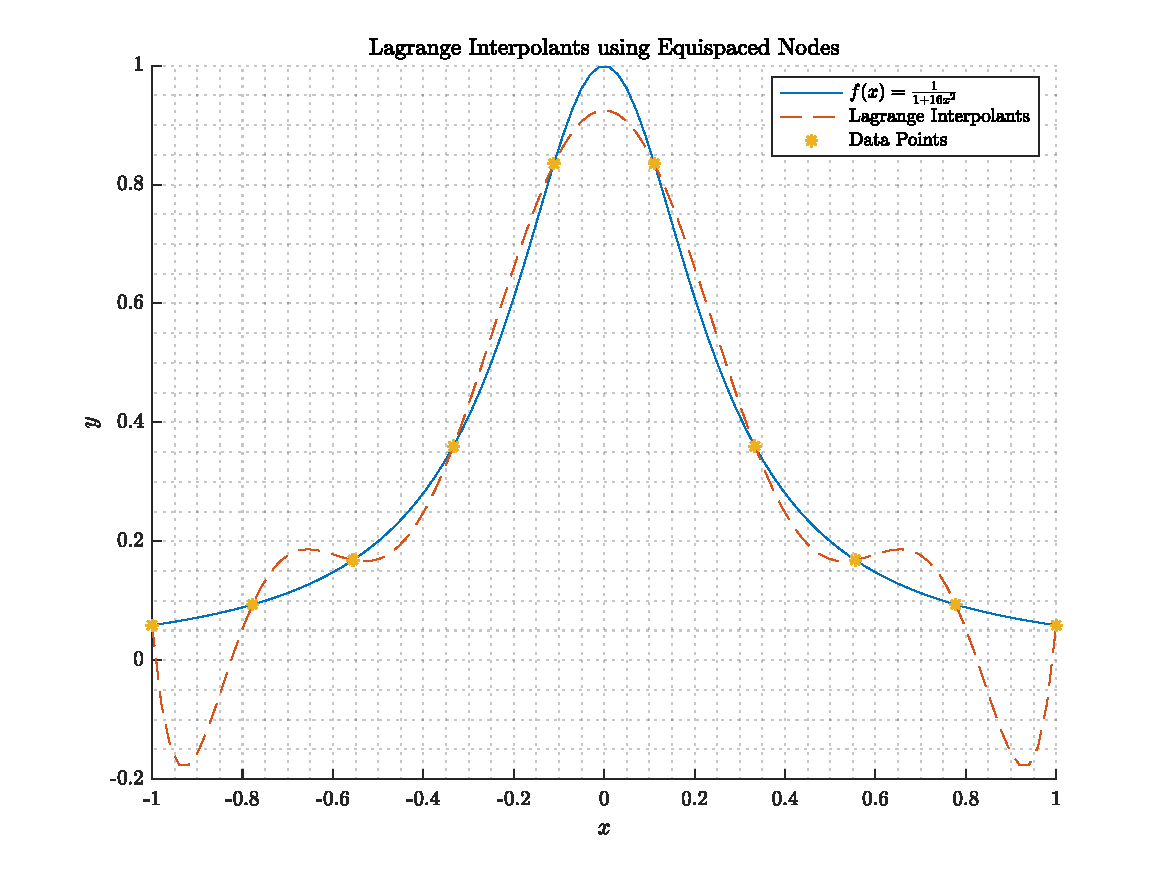
\includegraphics[width=0.75\linewidth]{../src/hw5_p1_b.pdf}
        \caption{Lagrange Interpolation for Equispaced Nodes}%
        \label{fig:p1b}
      \end{figure}
      \begin{figure}[!hbtp]
        \centering
        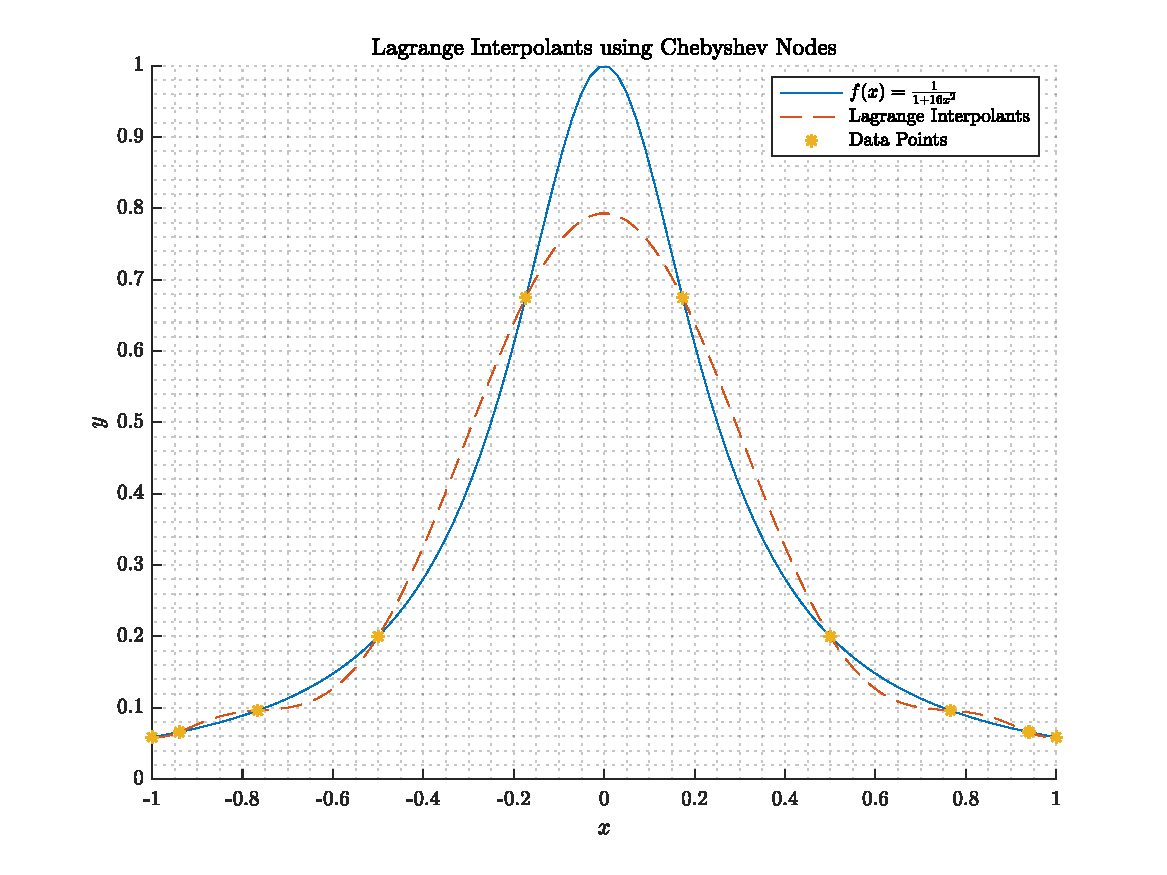
\includegraphics[width=0.75\linewidth]{../src/hw5_p1_c.pdf}
        \caption{Lagrange Interpolation for Chebyshev Nodes}%
        \label{fig:p1c}
      \end{figure}
  \end{itemize}
\end{solution}

%%%%%%%%%%%%%%%%%%%%%%%%%%%%%%%%%%%%%%%%%%%%%%%%
% Problem 2
%%%%%%%%%%%%%%%%%%%%%%%%%%%%%%%%%%%%%%%%%%%%%%%%
\section{Problem 2}%
\label{sec:problem_2}
This problem must be done by hand. Consider the data set
\begin{table}[!hbtp]
  \centering
  % \caption{}
  \label{tab:label}
  \begin{tabular}{ccccc}
    \toprule
    $k    $ & $0   $ & $1   $ & $2   $ & $3   $ \\
    \midrule
    $x_{k}$ & $0.1 $ & $0.3 $ & $0.5 $ & $0.7 $ \\
    $y_{k}$ & $1.01$ & $1.35$ & $2.11$ & $2.95$ \\
    \bottomrule
  \end{tabular}
\end{table}
and use it to approximate the value the function $y = f(x)$ at the point $x = 0.45$. To do this, construct the table of values $Q_{ij}(x)$ for the recursive pointwise evaluation of the interpretation polynomial (see the typed notes section 6.2.3, page 87 and following). Display all entries in your table with $3$ digit accuracy.
\begin{solution}
  The Lagrange Approximation is shown in Table \ref{tab:lagrange}.
  \begin{table}[!hbtp]
    \centering
    \caption{Lagrange Approximation to $y = f(x)$}
    \label{tab:lagrange}
    \begin{tabular}{c|c|C{3.3cm}|C{3.3cm}|C{3.3cm}|C{3.3cm}}
      \toprule
      $k$ & $x_{k}$ & $Q_{k0}$ & $Q_{k1}$ & $Q_{k2}$ & $Q_{k3}$ \\
      \midrule
      $0$ & $0.1$  & $1.0100$    & $     0$    & $     0$    & $     0$         \\
      $1$ & $0.3$  & $1.3500$    & $1.6050$    & $     0$    & $     0$         \\
      $2$ & $0.5$  & $2.1100$    & $1.9200$    & $1.8806$    & $     0$         \\
      $3$ & $0.7$  & $2.9500$    & $1.9000$    & $1.9125$    & $1.8992$         \\
      \bottomrule
    \end{tabular}
  \end{table}

  Here are detailed steps to obtain the table:
  \newpage \quad \vfill   % DELETE THIS LINE IF YOU TYPE THE ANSWER IN LaTeX
\end{solution}

%%%%%%%%%%%%%%%%%%%%%%%%%%%%%%%%%%%%%%%%%%%%%%%%
% Problem 3
%%%%%%%%%%%%%%%%%%%%%%%%%%%%%%%%%%%%%%%%%%%%%%%%
\section{Problem 3}%
\label{sec:problem_3}
This problem must also be done by hand. You again need to approximate the value of the same function $y = f(x)$, this time at the point $x = 0.35$. Using the same data set as in Problem 2 above, compute the complete table of Newton's divided differences and then construct the resulting interpolation polynomial. Use this polynomial to approximate $y = f(x)$ at the point $x = 0.35$.
\begin{solution}
  The approximation using Newton's divided-difference is shown in Table \ref{tab:newton}.
  \begin{table}[!hbtp]
    \centering
    \caption{Lagrange Approximation to $y = f(x)$}
    \label{tab:newton}
    \begin{tabular}{c|c|C{3.3cm}|C{3.3cm}|C{3.3cm}|C{3.3cm}}
      \toprule
      $k$ & $x_{k}$ & $f[x_{k}]$ & $f[x_{k - 1}, x_{k}]$ & $f[x_{k - 2}, x_{k - 1}, x_{k}]$ & $f[x_{k - 3}, x_{k - 2}, x_{k - 1}, x_{k}]$ \\
      \midrule
      $0$ & $0.1$  & $1.0100$    & $     0$    & $     0$   & $      0$  \\
      $1$ & $0.3$  & $1.3500$    & $1.7000$    & $     0$   & $      0$  \\
      $2$ & $0.5$  & $2.1100$    & $3.8000$    & $5.2500$   & $      0$  \\
      $3$ & $0.7$  & $2.9500$    & $4.2000$    & $1.0000$   & $-7.0833$  \\
      \bottomrule
    \end{tabular}
  \end{table}

  The resulting interpolation polynomial is
  \\[1cm]                   % DELETE THIS LINE IF YOU TYPE THE ANSWER IN LaTeX

  Therefore, the approximate value of $y = f(x)$ at $x = 0.35$ is
  \\[1cm]  $f(x) =   1.5139$.               % DELETE THIS LINE IF YOU TYPE THE ANSWER IN LaTeX

  Here are detailed steps to obtain the table:
  \newpage \quad \vfill     % DELETE THIS LINE IF YOU TYPE THE ANSWER IN LaTeX
\end{solution}

